\documentclass[12pt]{article}

\usepackage[a4paper, left=3cm, right=1.5cm, top=2cm, bottom=2cm]{geometry}

\setlength{\parindent}{1.25cm}

\usepackage[utf8]{inputenc}
\usepackage{mathtools}
\usepackage[russian, english]{babel}
\usepackage{multirow}
\usepackage{graphicx}
\usepackage{listings}
\usepackage{xcolor}
\usepackage{float}
\graphicspath{{/home/oriptal/Labs/Informatics/3. Regular Expressions (12.10.2024)/Report/files/}}

\addto\captionsenglish{\renewcommand{\contentsname}{\huge Table of Contents}}
\addto\captionsenglish{\renewcommand{\figurename}{Fig.}}

\begin{document}
	\begin{center}
		\thispagestyle{empty}
		\LARGE
		\textbf{NRU ITMO}\\
		SEaCT\\
		Informatics\\
	
		\vspace{7cm}
		
		\huge
		
		\textbf{Regular Expressions}\\
		Laboratory Work №3\\
		\vspace{1cm}
		\Large
		Variant 111
		
		\LARGE
		\vspace{5cm}
		\vbox{
			\hfill
			\vbox{
				\hbox{By: Loskutov P.\,A.}
				\hbox{To: Ponomarev V.\,V.}
			}
		} 
		
		\vspace{2.5cm}
		Saint Petersburg, 2024
		\newpage
		\tableofcontents
	\end{center}
	\newpage
	\Large
	\section{\LARGE Problems} 
	\begin{itemize}
		\item Determine variant by ISU number.
		\item Write the program, that can count amount of smile, that determine by variant.
		\item Write the program, that can delete repeating words from the text.
		\item Write the program, that put on output words, which has all the same vowels.
		\item Write 5 tests for each written program and prove results.
	\end{itemize}
	\newpage
	\section{\LARGE Solving}
	\subsection{\LARGE Variant}
	\begin{enumerate}
		\item My ISU = \(466537\)
		\item \(466537 \equiv 1(mod\; 6)\rightarrow\,\)Eyes is ``;``.
		\item \(466537 \equiv 1(mod\; 4)\rightarrow\,\)Nose is ``\(<\)``.
		\item \(466537 \equiv 1(mod\; 8)\rightarrow\,\)Mouth is ``)``.
		\item Then my smile is ``;\(<\))``.
	\end{enumerate}
	\subsection{\LARGE Programs}
	\begin{figure}[H]
		\setlength{\fboxsep}{0pt}
		\setlength{\fboxrule}{0pt}
		\begin{center}
			\lstset{language=python, numbers=left, showspaces=false,
				showstringspaces=false, tabsize=2, breaklines=true, keywordstyle=\color{magenta}}
			\begin{lstlisting}
				import re
				
				def count_smile(s: str)->int:
					regex = r';<\)'
					return len(re.findall(regex, s))
				
				
				def delete_repeating_words(s: str)->str:
					regex = r'(\w+)(?:\s+\1)+'
					return re.sub(regex, r'\1', s, flags=re.IGNORECASE)
				
				def find_one_vowel_words(s: str):
					vowels = russian_vowels
					non_vowels = russian_non_vowels
					regex = fr"\b[{non_vowels}]*([{vowels}])*(?:[{non_vowels}]*\1*)*\b"
					answer = []
					for sub in re.split(r'[-.;:\s|,|\*|\n]', s):
						if re.fullmatch(regex, sub, flags=re.IGNORECASE) is not None:
							answer.append(sub)
					answer.sort(key=lambda a: (len(a), a))
					return answer
			\end{lstlisting}
		\end{center}
	\end{figure}
	\newpage
	\subsection{\LARGE Tests}
	\subsubsection{\LARGE Main Quest}
	Input:
	\begin{figure}[H]
		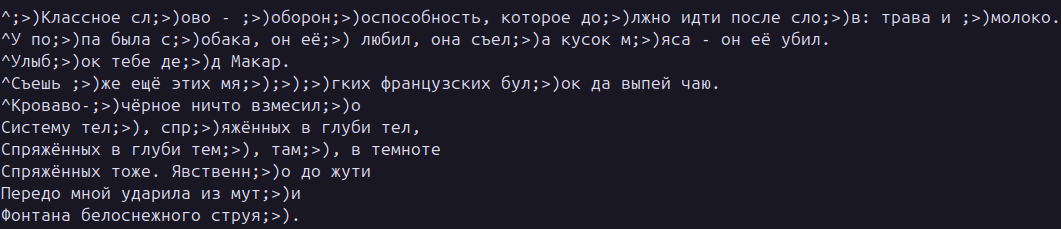
\includegraphics[scale=0.45]{60}
		\caption{The input for Main Quest.}
		\label{fig:60}
	\end{figure}
	Correct answers:
	\begin{enumerate}
		\item 7
		\item 5
		\item 2
		\item 5
		\item 9
	\end{enumerate}
	Output of program:
	\begin{figure}[H]
		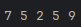
\includegraphics[scale=1]{output60}
		\label{fig:out60}
	\end{figure}
	\subsubsection{\LARGE Side Quest №1}
	Input:
	\begin{figure}[H]
		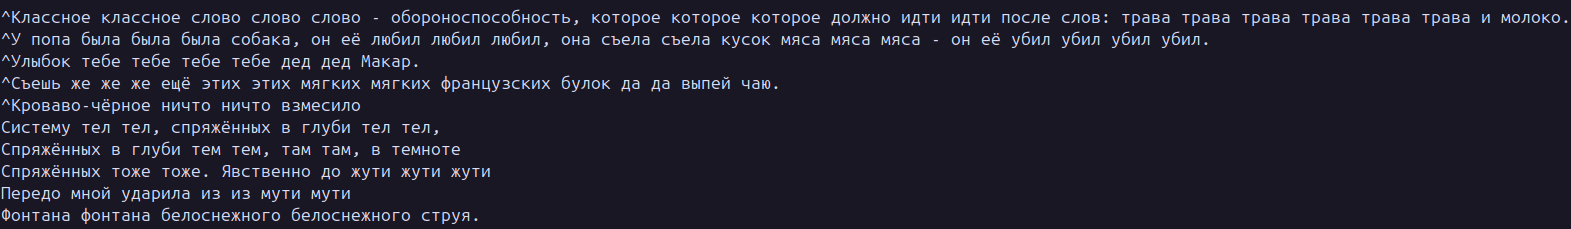
\includegraphics[scale=0.3]{18}
		\caption{The input for Side Quest №1.}
		\label{fig:18}
	\end{figure}
	Correct answers:
	\begin{figure}[H]
		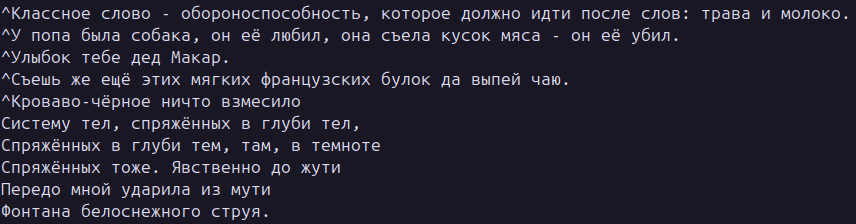
\includegraphics[scale=0.45]{corr18}
		\caption{The correct answer for Side Quest №1.}
		\label{fig:corr18}
	\end{figure}
	Output of program:
	\begin{figure}[H]
		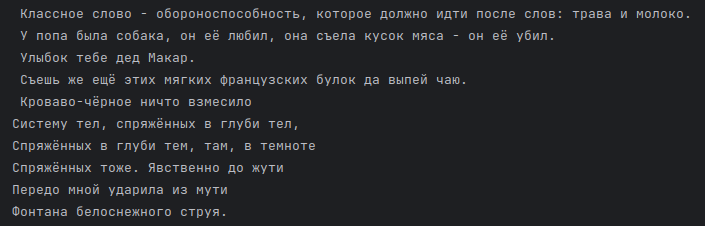
\includegraphics[scale=0.55]{output18}
		\label{fig:out18}
	\end{figure}
	\subsubsection{\LARGE Side Quest №2}
	Input:
	\begin{figure}[H]
		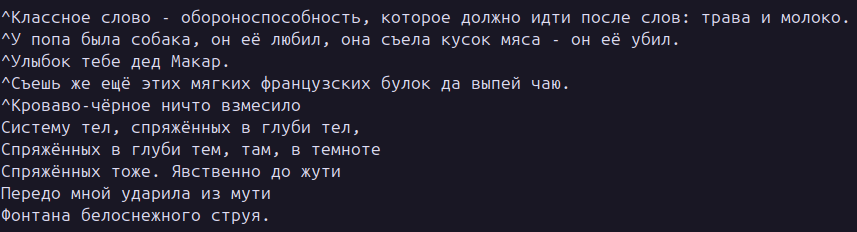
\includegraphics[scale=0.45]{22}
		\caption{The input for Side Quest №2.}
		\label{fig:22}
	\end{figure}
	Output of program:
	\begin{figure}[H]
		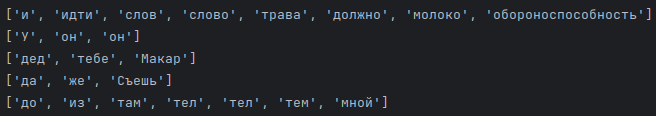
\includegraphics[scale=0.75]{output22}
		\label{fig:out22}
	\end{figure}
\end{document}

